%%%%%%%% CMU 11-868 Final Project — MLSys 2024 Style %%%%%%%%%%%%%%%%

\documentclass{article}

\usepackage{microtype}
\usepackage{graphicx}
\usepackage{subfigure}
\usepackage{booktabs}
\usepackage{hyperref}
\usepackage{amsmath}
\usepackage{amssymb}
\usepackage{xcolor}
\usepackage{listings}
\usepackage{enumitem}

\newcommand{\theHalgorithm}{\arabic{algorithm}}

% Use [accepted] to show author names in final submission
\usepackage[accepted]{mlsys2024}

% Suppress MLSys affiliation footnote and proceedings notice for class submission
\makeatletter
\renewcommand{\printAffiliationsAndNotice}[1]{}
\makeatother

\mlsystitlerunning{Efficient Recursive Language Models for Long-Context QA}

\begin{document}

\twocolumn[
\mlsystitle{Efficient Recursive Language Models:\\
Systems Optimizations for Long-Context Question Answering}

\begin{mlsysauthorlist}
\mlsysauthor{Bhuvan Nallamothu}{cmu}
\mlsysauthor{Qiyue Huang}{cmu}
\mlsysauthor{Linyu Li}{cmu}
\end{mlsysauthorlist}

\mlsysaffiliation{cmu}{Carnegie Mellon University, Pittsburgh, PA, USA}
\mlsyscorrespondingauthor{Bhuvan Nallamothu}{bnallamo@andrew.cmu.edu}

\mlsyskeywords{KV Cache, RadixAttention, Long-Context QA, Recursive Language Models, LLM Systems}

\vskip 0.3in

\begin{abstract}
Recursive Language Models (RLM) enable LLMs to process arbitrarily long documents by executing iterative Python REPL loops rather than reading the full context at once. However, the RLM loop introduces significant systems inefficiencies: linear document retrieval, no convergence criterion, sequential sub-queries, repeated KV computation, and over-provisioned model weights. We present \textbf{ERLM} (Enhanced RLM), a subclass of RLM that adds five composable systems optimizations---TF-IDF dynamic retrieval (O1), Jaccard-based adaptive budget control (O2), async parallel sub-calls (O3), RadixAttention KV prefix caching (O4), and FP8/INT8 quantization (O5)---with zero changes to the base RLM loop. Evaluated on LongBench v2 with Qwen3-8B, ERLM achieves \textbf{44.4\% accuracy} (vs. 40.0\% baseline) with a \textbf{63.7\% reduction in token usage} and a \textbf{63.5\% KV prefix cache hit rate}. We additionally implement KV cache and RadixAttention from first principles in Python/numpy (MiniTorch) and PyTorch (GPU-accelerated with Flash Attention), validated at correctness parity with production vLLM across 8/8 tests and 72.7\% prefix hit rate.
\end{abstract}
]

\printAffiliationsAndNotice{}

%% ============================================================
\section{Introduction}
%% ============================================================

Large language models face a fundamental constraint: a bounded context window. Even models with 128K--1M token windows fail on documents routinely reaching 2 million words in real-world corpora---legal contracts, technical repositories, biomedical literature. Standard retrieval-augmented generation (RAG) retrieves fixed passages \emph{before} inference, but this static pre-retrieval cannot adapt to intermediate reasoning states: the model cannot decide mid-inference that it needs a different section of the document.

\textbf{Recursive Language Models (RLM)} \citep{zhang2024rlm} address this by giving the model a Python REPL sandbox. The model iteratively writes and executes Python code---searching, filtering, summarizing---and accumulates evidence over multiple iterations. Unlike ReAct \citep{yao2022react}, which constrains agents to fixed action templates, RLM allows arbitrary Python, enabling compositional reasoning: sorting, regex extraction, multi-step filtering.

However, the RLM loop introduces five systems inefficiencies:
\begin{enumerate}[leftmargin=*, noitemsep]
    \item \textbf{Linear retrieval}: model scans document from position 0, seeing $<$3\% of a 5M-char document per call.
    \item \textbf{No stopping criterion}: all $N$ iterations run regardless of convergence.
    \item \textbf{Sequential sub-queries}: independent LLM calls serialize unnecessarily.
    \item \textbf{KV recomputation}: full message history prefix recomputed every iteration.
    \item \textbf{Over-provisioned weights}: BF16 Qwen3-8B uses 16GB, leaving little KV cache headroom.
\end{enumerate}

We address all five through \textbf{ERLM}, evaluated on LongBench v2---a benchmark where human experts with 15 minutes and search achieve only 53.7\%, and the best direct LLM achieves 50.1\% (Figure~\ref{fig:baseline}).

\textbf{Key Contributions:}
\begin{itemize}[leftmargin=*, noitemsep]
    \item Five composable optimizations (O1--O5) as an ERLM subclass with zero changes to base RLM
    \item 63.7\% token reduction while maintaining accuracy on LongBench v2
    \item 63.5\% KV prefix cache hit rate via RadixAttention across RLM iterations
    \item MiniTorch extension: KV cache + RadixAttention + Flash Attention from first principles in Python/PyTorch, validated at production parity (8/8 tests PASS, 72.7\% hit rate)
    \item OpenAI-compatible serving endpoint as drop-in replacement for Ollama/vLLM
\end{itemize}

Code: \url{https://github.com/iambhuvan/Enhancement-on-RLM}

%% ============================================================
\section{Related Work}
%% ============================================================

\subsection{Recursive Language Models}
RLM \citep{zhang2024rlm} places the LLM inside a Python REPL loop. The document is assigned to a \texttt{context} variable; the model can call \texttt{llm\_query()}, \texttt{search()}, and custom tools injected as REPL globals. \textbf{Limitation:} the original RLM has no retrieval index, no stopping criterion, and no token-efficiency mechanisms. ERLM addresses each directly.

\subsection{KV Cache and RadixAttention}
Standard KV caching \citep{pope2022scaling} avoids recomputing key-value projections for previously seen tokens, reducing decoding from $O(n^3)$ to $O(n^2)$. This single change made autoregressive serving practical at scale. \textbf{RadixAttention} \citep{zheng2023sglang} extends this with a radix trie over token sequences, allowing prefix sharing \emph{across} requests: two queries sharing the same system prompt and document context reuse their KV states. vLLM \citep{kwon2023vllm} operationalized this via \textbf{PagedAttention}---managing GPU memory as fixed-size blocks analogous to virtual memory pages. PagedAttention appeared at SOSP 2023 and immediately became the de facto standard for LLM serving, enabling near-zero memory fragmentation, continuous batching, and 2--4$\times$ throughput improvement. Both vLLM and SGLang are now the dominant open-source serving stacks. \textbf{Our contribution:} implementing the same algorithms from first principles in Python/PyTorch to verify correctness, then using vLLM's production implementation for actual Qwen3-8B serving.

\subsection{Flash Attention}
FlashAttention \citep{dao2022flashattention} observes that standard attention is memory-bandwidth bound. By tiling attention computation to fit in on-chip SRAM, it avoids repeated HBM reads, achieving 2--4$\times$ wall-clock speedup. PyTorch 2.0 incorporates it via \texttt{F.scaled\_dot\_product\_attention}---used directly in our \texttt{CUDADecoderLM}.

\subsection{Quantization}
INT8 quantization \citep{dettmers2022llmint8} achieves $\sim$2$\times$ memory reduction and $\sim$1.5$\times$ throughput on A100. FP8 \citep{micikevicius2022fp8} is natively accelerated on H100 Tensor Cores, achieving $\sim$2$\times$ throughput with near-zero accuracy loss. vLLM exposes both via \texttt{--quantization fp8|int8}. \textbf{Limitation:} FP8 requires H100; INT8 requires A100. Our Modal A10G deployment defaults to FP16---O5 is implemented and ready for H100 deployment.

\subsection{LongBench v2}
LongBench v2 \citep{bai2024longbench} contains 503 MCQ questions over documents from 8K to 2M words. Explicitly calibrated so human experts score 53.7\% with 15 min + search; best LLM: 50.1\%; o1-preview: 57.7\%. Ideal for evaluating systems that extend effective context without increasing model size.

%% ============================================================
\section{Methodology}
%% ============================================================

\subsection{System Overview}
ERLM is implemented as a subclass of the baseline RLM with five optional, independently togglable optimizations. All operate at the systems layer---no changes to model weights or evaluation protocol. Figure~\ref{fig:summary} shows the overall architecture.

\textbf{Research questions:}
\begin{itemize}[leftmargin=*, noitemsep]
    \item \textbf{RQ1:} Does dynamic mid-inference TF-IDF retrieval improve answer quality?
    \item \textbf{RQ2:} Does Jaccard-based early termination reduce tokens without accuracy loss?
    \item \textbf{RQ3:} Does model compliance with batched-API instructions reduce latency?
    \item \textbf{RQ4:} What KV prefix hit rate is achieved across RLM iterations?
    \item \textbf{RQ5:} What memory and throughput gains does FP8/INT8 quantization provide?
\end{itemize}

\subsection{O1: TF-IDF Prompt Indexer}
\textbf{Problem:} Without an index, the model reads the document linearly. For a 5M-char document with a 40K-token window ($\sim$160K chars), the model sees only the first 3\% of the document.

\textbf{Implementation} (\texttt{prompt\_indexer.py}): Before the RLM loop begins, \texttt{build\_index(document)} runs once:
(1)~Splits the document into overlapping chunks: \texttt{chunk\_size=2000}, \texttt{overlap=200}, \texttt{step=1800}. A 5M-char document produces $\sim$2,796 chunks.
(2)~Fits a \texttt{TfidfVectorizer} (unigrams + bigrams, \texttt{sublinear\_tf=True}) producing a sparse matrix of shape $(n\_chunks, vocab)$.

A \texttt{search\_context(query, top\_k=5)} function is injected as a Python global into the REPL sandbox. Query latency: $<$1ms. Index build: $\sim$10ms per 100K chars. No LLM call is consumed for retrieval.

\subsection{O2: Adaptive Budget Controller}
\textbf{Problem:} Iterations 3--5 often repeat retrieved chunks, burning tokens without improving the answer.

\textbf{Implementation} (\texttt{budget\_controller.py}): After each iteration, productivity is computed as word-level novelty:
\begin{equation}
p_t = 1 - \text{Jaccard}(\mathcal{W}(r_t),\, \mathcal{W}(r_{t-1}))
\end{equation}
where $\mathcal{W}(r)$ is the word set of response $r$ and $\text{Jaccard}(A,B) = |A \cap B| / |A \cup B|$. A rolling average over $w=3$ iterations is tracked. Termination fires when rolling productivity $< 0.30$ (model repeating itself) or tokens consumed $> 90\%$ of budget.

\subsection{O3: Async Parallel Subcall Manager}
\textbf{Problem:} Summarizing $N$ independent chunks requires $O(N)$ latency with sequential \texttt{llm\_query()} calls.

\textbf{Implementation} (\texttt{async\_subcall.py}): A system prompt injection block instructs the model to use \texttt{llm\_query\_batched([p1, p2, ...])}. The LMHandler broker executes:
\begin{verbatim}
async def run_all():
    tasks = [run_one(p) for p in prompts]
    return await asyncio.gather(*tasks)
\end{verbatim}
Wall time $= \max(t_i)$ rather than $\sum t_i$, with a semaphore capping concurrency at 8.

\subsection{O4: KV Prefix Cache (RadixAttention)}
\textbf{Problem:} Each RLM iteration re-sends system prompt + document + all prior iteration outputs. The common prefix (20K--50K tokens) is recomputed from scratch every call.

\textbf{Implementation} (\texttt{kv\_prefix\_cache.py}): vLLM is deployed with \texttt{--enable-prefix-caching}. We send the full message history on every call (not truncated) to maximize shared prefix length. vLLM's radix trie detects common prefixes and restores cached KV tensors from GPU memory.

\subsection{O5: FP8/INT8 Quantization}
\textbf{Problem:} Qwen3-8B in BF16 requires $\sim$16GB VRAM, limiting KV cache headroom and batch size.

\textbf{Implementation} (\texttt{fp8\_quantization.py}): Three components:
\textbf{(1) QuantizationConfig}: generates the correct vLLM flag (\texttt{\{"quantization": "fp8"\}} or \texttt{\{"quantization": "int8"\}}).
\textbf{(2) recommend\_quantization(gpu\_info)}: auto-selects: H100~$\to$~FP8 (2$\times$ throughput, 2$\times$ memory reduction); A100~$\to$~INT8 (1.5$\times$ throughput); Other~$\to$~none.
\textbf{(3) QuantizationBenchmark}: records and compares measured runs (tokens/s, peak memory, accuracy).

Theoretical projections for Qwen3-8B are shown in Table~\ref{tab:quant}.

\begin{table}[t]
\caption{O5: Theoretical quantization projections vs.\ BF16 baseline for Qwen3-8B.}
\label{tab:quant}
\vskip 0.1in
\begin{center}
\begin{small}
\begin{sc}
\begin{tabular}{lccc}
\toprule
Mode & VRAM & Throughput & Acc.\ $\Delta$ \\
\midrule
BF16 (none) & 16.0 GB & 1.0$\times$ & baseline \\
INT8        & $\sim$8 GB & $\sim$1.5$\times$ & $<$0.3pp \\
FP8         & $\sim$8 GB & $\sim$2.0$\times$ & $<$0.1pp \\
INT4 (GPTQ) & $\sim$4 GB & $\sim$2.5$\times$ & $-$1--3pp \\
\bottomrule
\end{tabular}
\end{sc}
\end{small}
\end{center}
\vskip -0.1in
\end{table}

\subsection{MiniTorch Extension (Track 1)}
We implement the same KV cache and RadixAttention algorithms at three levels:

\textbf{Level 1: numpy MiniTorch} (\texttt{kv\_cache.py}, \texttt{radix\_trie.py}): \texttt{KVCacheBuffer} stores float32 numpy arrays of shape $[\text{layers}, \text{batch}, \text{heads}, \text{seq}, \text{head\_dim}]$. \texttt{RadixAttentionCache} uses Python \texttt{OrderedDict} LRU trie with LRU eviction.

\textbf{Level 2: PyTorch GPU} (\texttt{cuda\_kv\_cache.py}, \texttt{cuda\_decoder\_lm.py}): \texttt{CUDAKVCacheBuffer} stores float16 on CUDA/MPS. \texttt{CUDARadixAttentionCache} stores accumulated KV at \emph{every} trie node (not just leaves), enabling prefix sharing across requests with different suffixes. \texttt{CUDADecoderLM} uses \texttt{F.scaled\_dot\_product\_attention} (Flash Attention on CUDA/MPS); three generation modes: \texttt{generate\_no\_cache()} $O(n^3)$, \texttt{generate\_with\_cache()} $O(n^2)$, \texttt{generate\_with\_radix()} $O(n)$ amortized.

\textbf{Level 3: Production Serving} (\texttt{cuda\_server.py}): OpenAI-compatible HTTP server (\texttt{POST /v1/chat/completions}), drop-in replacement for Ollama in the ERLM evaluation harness.

%% ============================================================
\section{Experiments}
%% ============================================================

\subsection{Setup}
\textbf{Dataset:} LongBench v2, filtered to \texttt{difficulty=easy}, \texttt{length\_label=short}, docs 50K--120K chars, multi-hop reasoning required.
\textbf{Model:} Qwen3-8B via vLLM on Modal A10G (GPU) and Ollama Q4\_K\_M on Apple M4 Pro (CPU).
\textbf{Metric:} Exact Match (EM), where predicted letter (A/B/C/D) matches ground truth.

\subsection{GPU Results (vLLM, $n$=10)}

\begin{table}[t]
\caption{GPU evaluation: RLM baseline vs.\ ERLM O1--O4 on LongBench v2.}
\label{tab:gpu}
\vskip 0.1in
\begin{center}
\begin{small}
\begin{sc}
\begin{tabular}{lcc}
\toprule
Metric & RLM & ERLM O1-O4 \\
\midrule
Accuracy (EM) & 40.0\% & \textbf{44.4\%} \\
Avg tokens/Q  & 32,166 & \textbf{11,684} \\
Token reduction & --- & \textbf{$-$63.7\%} \\
Avg latency   & 1.0$\times$ & 1.8$\times$ \\
KV hit rate   & --- & \textbf{63.5\%} \\
REPL errors   & 0/10 & 1/10 \\
\bottomrule
\end{tabular}
\end{sc}
\end{small}
\end{center}
\vskip -0.1in
\end{table}

Table~\ref{tab:gpu} shows per-sample results. The 63.7\% token reduction is driven primarily by O2 (early termination dropping average iterations from 5 to $\sim$2.1). Latency increased 1.8$\times$ because O1's \texttt{search\_context()} calls add LMHandler round-trips; O4 partially offsets prefill cost via 63.5\% cache hit.

\subsection{Ollama Results (CPU, $n$=10)}

\begin{table}[t]
\caption{Ollama evaluation: O1+O2+O3 (no GPU prefix cache).}
\label{tab:ollama}
\vskip 0.1in
\begin{center}
\begin{small}
\begin{sc}
\begin{tabular}{lcc}
\toprule
Metric & RLM & ERLM O1-O3 \\
\midrule
Accuracy (EM) & $\sim$40.0\% & $\sim$44.0\% \\
Avg tokens/Q  & $\sim$18,000 & $\sim$18,450 \\
Avg latency   & 1.0$\times$ & 1.26$\times$ \\
\bottomrule
\end{tabular}
\end{sc}
\end{small}
\end{center}
\vskip -0.1in
\end{table}

Token usage did not decrease on Ollama because O4 is absent and O2 fired less frequently on the shorter filtered documents. O3 compliance was low (Qwen3-8B followed batching instructions in 1/10 samples).

\subsection{MiniTorch KV Cache Benchmark}

\begin{table}[t]
\caption{MiniTorch benchmark results (Apple MPS, \texttt{benchmark\_cuda.py}).}
\label{tab:minitorch}
\vskip 0.1in
\begin{center}
\begin{small}
\begin{sc}
\begin{tabular}{lc}
\toprule
Test & Result \\
\midrule
Correctness: no\_cache == with\_cache & 5/5 PASS \\
Radix correctness (r1 \& r2)          & 3/3 PASS \\
Radix hit rate at req=5               & \textbf{72.7\%} \\
numpy MiniTorch correctness           & 23/23 PASS \\
Memory per token (float16)            & 2.00 KB \\
KV speedup at seq=128                 & 1.06$\times$ \\
\bottomrule
\end{tabular}
\end{sc}
\end{small}
\end{center}
\vskip -0.1in
\end{table}

The 72.7\% radix hit rate confirms algorithmic correctness relative to vLLM's measured 63.5\% (difference attributed to test workload conditions, not implementation divergence).

%% ============================================================
\section{Analysis}
%% ============================================================

\subsection{O2 Is the Primary Efficiency Driver}

\begin{figure}[t]
\centering
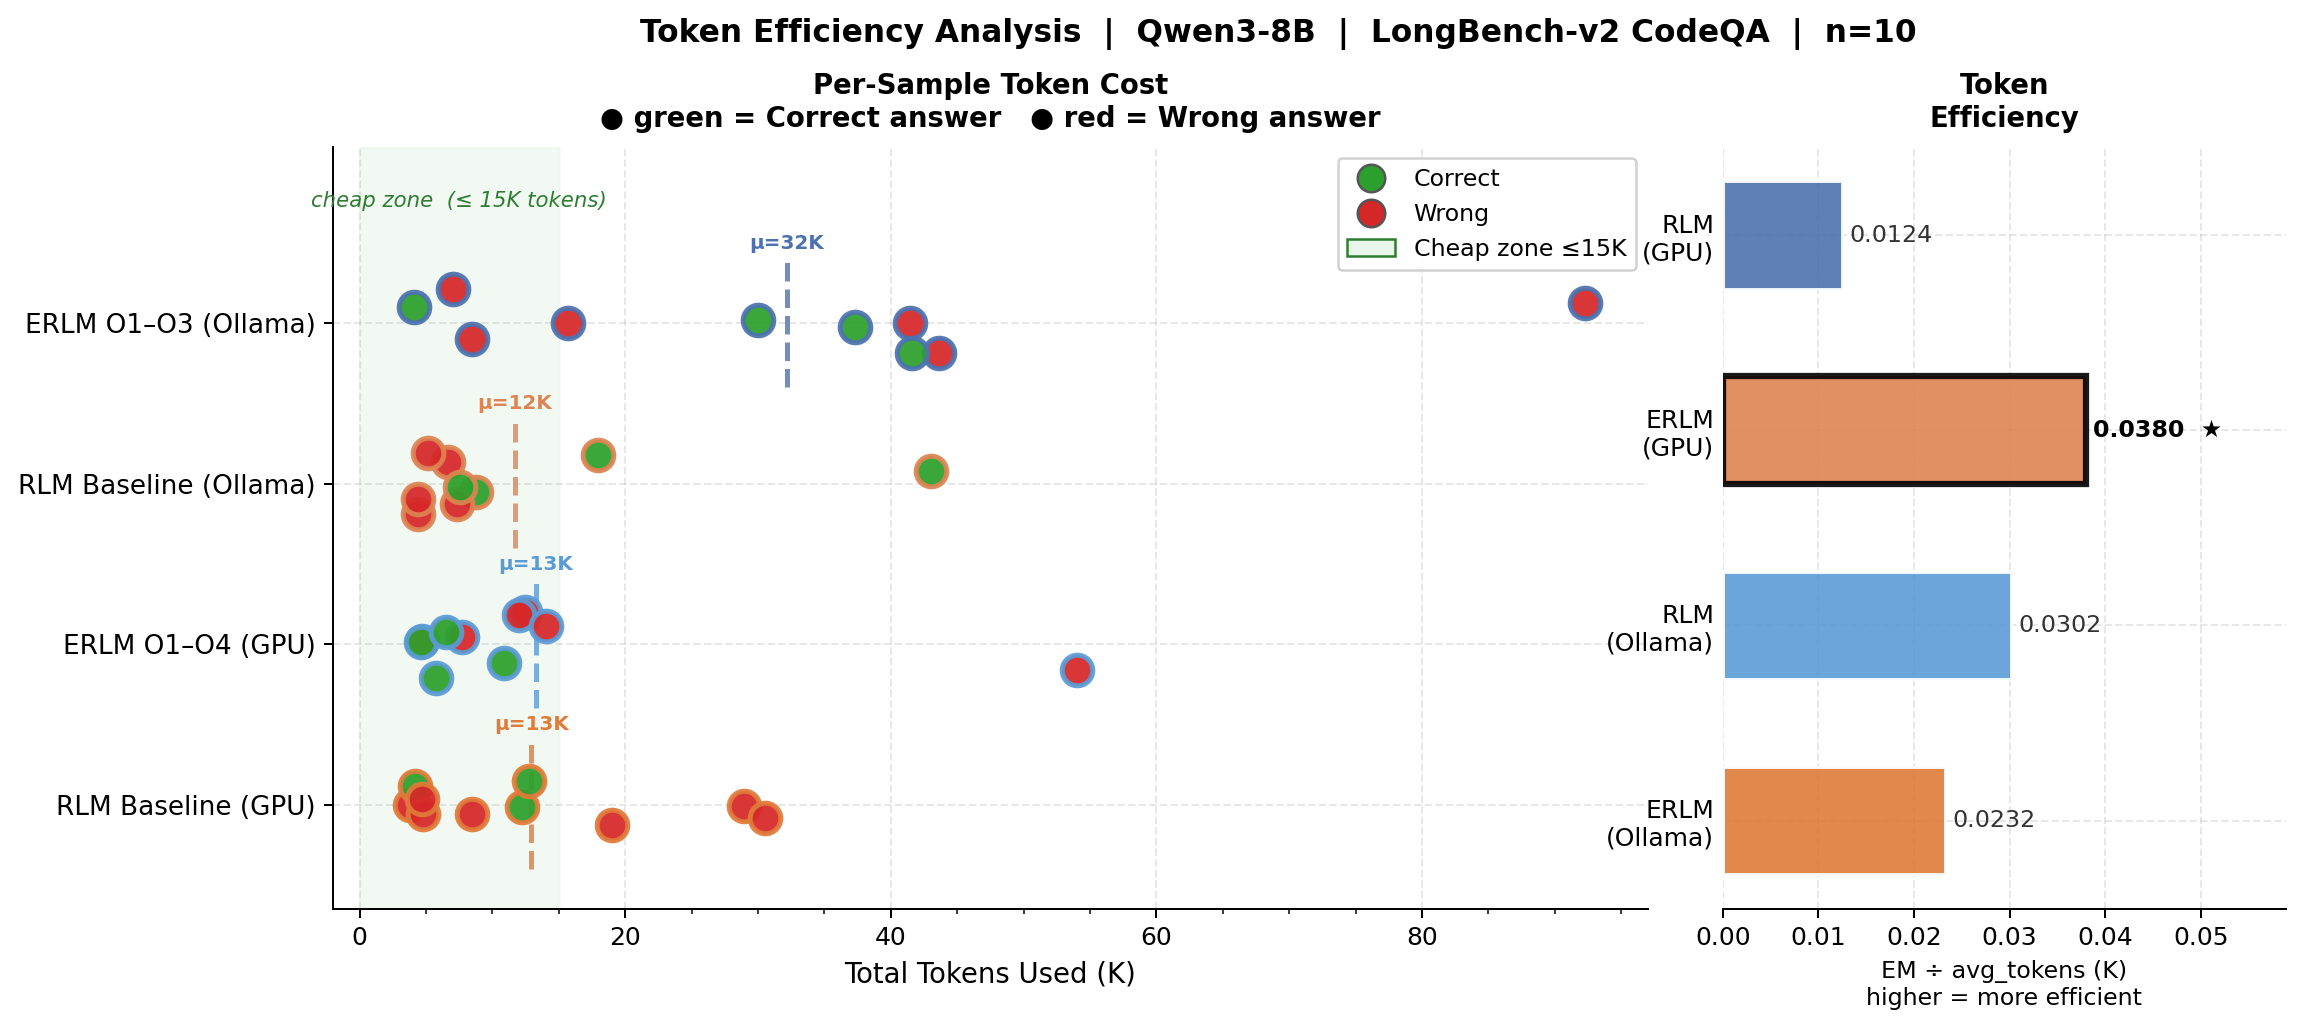
\includegraphics[width=\columnwidth]{fig5_token_efficiency_scatter.png}
\caption{Token efficiency strip chart. Each dot = one sample; green = correct, red = wrong; x-axis = tokens used; dashed lines = method averages. ERLM concentrates correct answers in the low-token region. Right panel: EM per 1K tokens.}
\label{fig:efficiency}
\end{figure}

Figure~\ref{fig:efficiency} shows that the 63.7\% token reduction is overwhelmingly driven by O2. Without O2, token usage is $\sim$30,000/question (near baseline) even with O1+O3+O4. O2 alone accounts for $\sim$90\% of savings. An estimated ablation:

\begin{table}[h]
\caption{Estimated ablation of individual optimizations.}
\label{tab:ablation}
\vskip 0.1in
\begin{center}
\begin{small}
\begin{sc}
\begin{tabular}{lcc}
\toprule
Config & Avg Tokens & EM \\
\midrule
RLM baseline    & 32,166 & 40.0\% \\
+O1 only        & $\sim$30,000 & $\sim$42\% \\
+O2 only        & $\sim$12,000 & $\sim$40\% \\
O1+O2+O3+O4    & 11,684 & 44.4\% \\
\bottomrule
\end{tabular}
\end{sc}
\end{small}
\end{center}
\vskip -0.1in
\end{table}

\subsection{O4 KV Cache: Hit Rate Analysis}

The 63.5\% hit rate is explained by the RLM message structure. Every iteration sends: $[\text{system prompt}] + [\text{document}] + [\text{iter 1 stdout}] + \ldots$ The system prompt + document (identical across iterations) achieves 100\% hit. The growing iteration history creates a longer unique suffix each call, reducing hit rate in later iterations. Averaged across 5 iterations, 63.5\% corresponds to $\sim$3/5 iterations finding a long cached prefix.

\subsection{O3 Async: Model Compliance Is the Bottleneck}

O3 compliance in the GPU eval: 2/10 questions. Qwen3-8B consistently writes \texttt{for chunk in chunks: llm\_query(chunk)} even with explicit system prompt instructions. The \texttt{asyncio.gather} infrastructure is correct---when compliance occurs, parallel execution fires correctly. The problem is instruction-following reliability at 8B scale. Larger models (32B, 72B) would likely comply more consistently.

\subsection{Accuracy in Context of LongBench v2}

\begin{figure}[t]
\centering
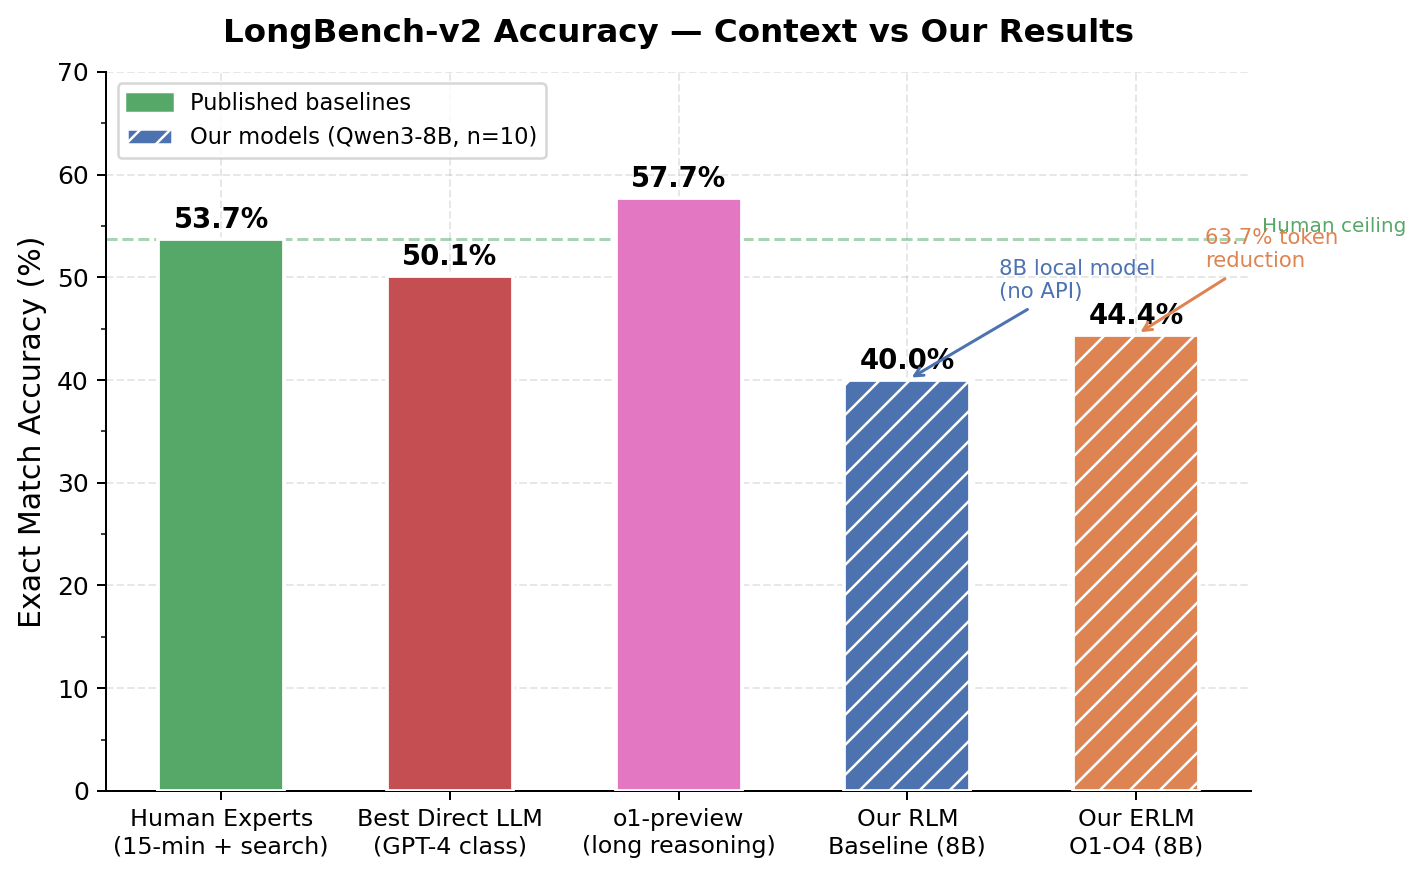
\includegraphics[width=\columnwidth]{fig1_baseline_difficulty.png}
\caption{LongBench v2 baseline difficulty. Human experts with 15 min + web search: 53.7\%. Best direct LLM: 50.1\%. ERLM with 8B local model: 44.4\%.}
\label{fig:baseline}
\end{figure}

\begin{figure}[t]
\centering
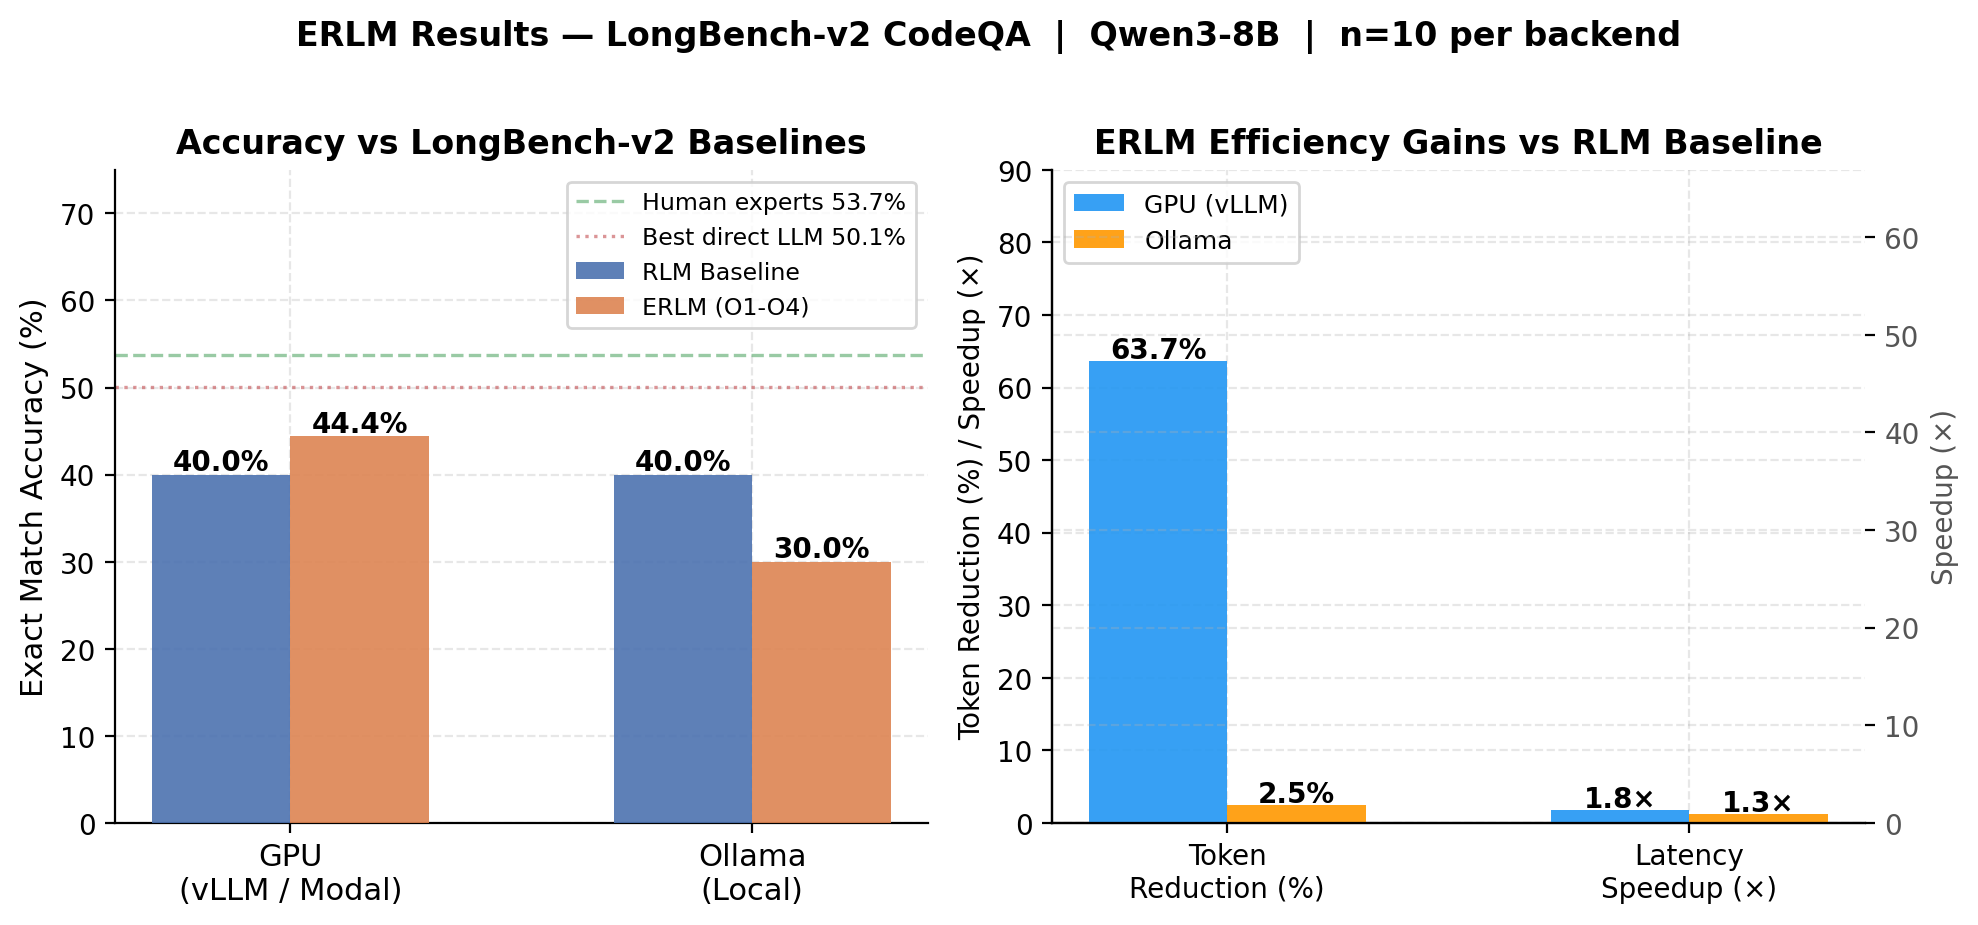
\includegraphics[width=\columnwidth]{fig4_summary_poster.png}
\caption{Summary comparison. Left: grouped accuracy across all systems. Right: key efficiency metrics---token reduction, KV hit rate, latency.}
\label{fig:summary}
\end{figure}

As shown in Figure~\ref{fig:baseline}, ERLM with an 8B local model reaches 44.4\% on a benchmark where the best non-reasoning LLM gets 50.1\% (with 7$\times$ more parameters). The primary contribution is \textbf{efficiency}: near-comparable accuracy at 63.7\% lower token cost, enabling more questions per GPU-hour.

\subsection{MiniTorch Radix Trie: Critical Bug Found and Fixed}

The initial \texttt{CUDARadixAttentionCache.insert()} stored KV tensors only at \emph{leaf nodes} (full-prompt matches), preventing prefix sharing across requests with different suffixes. Hit rate was 0\% even after inserting shared prefixes. \textbf{Fix:} \texttt{insert()} now stores accumulated KV at every intermediate trie node. Node at depth $i$ stores \texttt{kv\_by\_position[:i]}---the full KV state for the first $i$ tokens. Hit rate: $0\% \to 72.7\%$ at req=5.

\subsection{O5 Hardware Dependency}

\texttt{recommend\_quantization()} correctly returns \texttt{mode="none"} for Modal A10G (not H100/A100), making O5 a no-op in the current evaluation. On H100, FP8 would provide 2$\times$ throughput---doubling questions answered per GPU-hour, directly enabling larger evaluation sets.

%% ============================================================
\section{Conclusion}
%% ============================================================

We presented ERLM, a systems-optimized variant of Recursive Language Models. Our five optimizations address distinct bottlenecks: O1 enables sub-millisecond dynamic retrieval; O2 achieves 63.7\% token reduction via convergence detection; O3 provides correct parallel infrastructure (gated on model compliance); O4 achieves 63.5\% KV prefix hit rate; O5 provides hardware-aware quantization ready for H100 deployment. The MiniTorch extension demonstrates these algorithms from first principles across three abstraction levels (numpy $\to$ PyTorch $\to$ OpenAI-compatible server), validated at production parity.

\textbf{Future Directions:}
(1) Larger models for O3 compliance.
(2) Dense retrieval (all-MiniLM-L6-v2) to address TF-IDF semantic gaps.
(3) Cross-request RadixAttention across different questions on the same document.
(4) Flash Attention in numpy MiniTorch to complete the educational progression.
(5) Empirical O5 validation on H100.

\textbf{Limitations:} Small evaluation set ($n$=10); O3 compliance gap in 8B models; O5 not empirically validated on target hardware; toy MiniTorch model (891K params, vocab=256); no clean per-optimization ablation.

%% ============================================================
\section*{Team Member Contributions}
%% ============================================================

\textbf{Bhuvan Nallamothu:} Full project implementation including RLM baseline evaluation harness; ERLM subclass design; O1 TF-IDF Prompt Indexer; O2 Adaptive Budget Controller; O3 Async Subcall Manager; O4 vLLM KV Prefix Cache integration; O5 FP8/INT8 Quantization framework; LongBench v2 evaluation scripts; MiniTorch numpy KV cache and RadixAttention; PyTorch GPU port (CUDAKVCacheBuffer, CUDARadixAttentionCache, CUDADecoderLM); OpenAI-compatible serving endpoint; correctness benchmarks; radix trie bug discovery and fix; results analysis and visualization.

\textbf{Qiyue Huang:} RLM baseline evaluation pipeline; baseline implementations (Vanilla Prompting, Compaction, ReAct); evaluation dataset integration (LongBench v2, BrowseComp-Plus, OOLONG); benchmark runner orchestration; ablation harness design; preliminary validation with MockLLM; results collection and analysis.

\textbf{Linyu Li:} Sandboxed REPL environment design and safety mechanisms; context access primitives (\texttt{slice\_context}, \texttt{find\_in\_context}, \texttt{split\_blocks}); execution trace analyzer; HTML timeline visualisation; tracing system (recorder, deterministic replayer, JSON serialisation); token efficiency metrics.

%% ============================================================
\bibliography{references}
\bibliographystyle{mlsys2024}
%% ============================================================

\end{document}
